\documentclass[a4paper,openany,12pt]{book}
\usepackage[spanish]{babel}
\usepackage[utf8]{inputenc}
\usepackage{graphicx}
\usepackage{amsmath}
\usepackage{amsfonts}
\usepackage{fancyhdr}
\usepackage{ae}
\usepackage[left=2.5cm,right=2.5cm,top=3cm,bottom=3cm]{geometry}
\usepackage[printonlyused]{acronym}
\usepackage{hlundef}
\usepackage{tesis}

\title{Deep Q-Learning multiagente aplicado a la creación de un equipo de fútbol de agentes simulados 2D}

\author{José Enrique Carrillo Pino}

\orientador{Prof Dr. Dennis Barrios Aranibar}

\dedicado{Dedico este trabajo a mis padres, por todo el esfuerzo que han hecho en sacarme adelante y a mis profesores por todas sus enseñanzas.}

\begin{document}
\maketitle %Compone la carátula y la dedicatoria

%mayores detalles de como usas las abreviaturas (acronimos)
% vea: http://www.ctan.org/tex-archive/macros/latex/contrib/acronym/
% hay un manual en pdf en esa misma direccion

\chapter*{Abreviaturas}

\begin{acronym}
\acro{RL}{Reinforcement Learning}
\acro{MDP}{Markov Decision Process}
\acro{GPI}{Generalized Policy Iteration}
\acro{DPG}{Deterministic Policy Gradient}
\acro{DQN}{Deep Q-Network}
\acro{DBN}{Deep Belief Network}
\acro{RBM}{Restricted Boltzman Machine}
\acro{MLP}{Multilayer Perceptron}
\acro{CNN}{Convolusional Neural Network}

\acro{SPC}{Sociedad Peruana de Computación}
\acro{CMM}{\textit{Capability Maturity Model}}
\end{acronym}

\begin{agradecimientos}
Aqu� deber�s colocar a quien y porque agradeces. Ejemplo:

En primer lugar deseo agradecer a Dios por haberme guiado a lo largo de estos cinco a�os de estudio.

Agradezco a mis padres por el apoyo brindado para forjarme como un profesional.

Agradezco a la universidad, mi \textit{alma matter}, por haberme cobijado y brindado la formaci�n que ahora me permitir� ayudar a construir una mejor sociedad.

Agradezco de forma muy especial a mi orientador Prof. Dr./Mag. nombre 1 por haberme guiado en esta tesis. ...

Deseo agradecer de forma especial a mis docentes: nombre 1, nombre 2, nombre 3 porque fueron ejemplos que deseo seguir en mi vida profesional.

Deseo agradecer al personal administrativo de la universidad: nombre 1, nombre 2, nombre 3. Muchas gracias por la atenci�n brindada y porque siempre estuvieron dispuestas a ayudarnos.
\end{agradecimientos}
 %Inserta los agradecimientos
\begin{resumen}
Aqu� deber�s colocar entre 100 y 150 palabras como
m�ximo, el problema que intentas resolver, la
justificaci�n y los aportes o soluciones que planteas.
\end{resumen}
 %Inserta el resumen
\begin{abstract}
Reinforcement Learning now has more attention due to the introduction of Deep Q Network. As a result there are many investigation lines currently. In the other hand, RoboCup has a soccer simulation 2D category that stimulates and let test new ideas in the field of artificial intelligence. In this work we propose the creation of a simulated soccer team using Deep Q Network algorithm. This is interesting and challenging because we have to use cooperative learning techniques from multiagent systems as well. This way, we hope to get a little bit closer to reach the goal of RoboCup: to play with the world champion soccer team with a robotic team in 2050 and win. In this work, we hope that our team plays at least better than a standard team called agent2d.
\end{abstract}
 %Inserta el abstract

\tableofcontents %Inserta el índice general
\listoftables %Inserta el índice de cuadros
\listoffigures %Inserta el índice de figuras

%%%%%%%%%%%%%%%%%%%%%%%%%%%%%%%%%%%%%%%%%%%%%%%%%%%%%%%%%%%%%%%%%%%%%
%%%%   En esta parte deberas incluir los archivos de tu tesis   %%%%%
%%%%%%%%%%%%%%%%%%%%%%%%%%%%%%%%%%%%%%%%%%%%%%%%%%%%%%%%%%%%%%%%%%%%%

\chapter{Introducción}

% Tengo 2 opciones:
% Usar la comparacion como centro del trabajo, pero no tiene mucho sentido, puesto que ya se sabe que dqn es mejor. No hay mucho q comparar
% Queda: Ejecutar una tecnica reciente en un problema importante y describir resultados, comparar con el estado del arte
%


\section{Motivación y Contexto}

La robocup tiene como objectivo construir un equipo robótico capaz de jugar fútbol con el campeón mundial y ganar en el año 2050. Con este fin se tienen varias categorias de competición que retan a los investigadores de todo el mundo para ir mejorando poco a poco los algoritmos y técnicas utilizadas en la construcción de robots.

Una de esas categorías es la simulación de fútbol 2D, que como su nombre lo indica es una simulación. La ventaja de una simulación es que abstrae todos los detalles de construcción del hardware de los robots y permite a los investigadores centrarse en los algoritmos, en la estrategia. Gracias a esto, esta categoría sirve como una cama de pruebas muy interesante para probar algoritmos de inteligencia artificial nuevos.

Recientemente se anunció la noticia de que finalmente se había creado una inteligencia artificial capaz de ganarle al campeón mundial de Go en una ronda de 5 partidas, donde quedaron 4 contra 1. El algoritmo que logró esta hazaña combina 2 grandes ramas de la inteligencia artificial: el aprendizaje por refuerzo y el aprendizaje profundo. Con este mismo algoritmo también se creó una inteligencia artificial capaz de aprender a jugar 49 juegos de Atari teniendo como entrada solamente los píxeles de la pantalla y la puntuación.

En este trabajo se pretende dar un paso inicial hacia la creación de un equipo robotico simulado, utilizando un algoritmo del estado del arte actual, como es el aprendizaje por refuerzo profundo.


\section{Planteamiento del Problema}

El fútbol de robots simulado es un problema muy difícil que se puede modelar con un \ac{MDP} con número de estados virtualmente infinito. El problema que se quiere abordar en este proyecto es el aprendizaje de jugadas individuales de un agente en la modalidad de aprendizaje por refuerzo.


\section{Objetivos}

Que un agente aprenda a esquivar rivales y anotar goles usando un algoritmo de aprendizaje por refuerzo profundo.


\subsection{Objetivos Específicos}

\begin{itemize}
\item Modelar el problema como un \ac{MDP} con sus respectivos estados, acciones y función de recompensa
\item Implementar el algoritmo \ac{DQN} en un agente y entrenarlo
\item Analizar el desempeño del agente en la tarea dada
\end{itemize}


\section{Organización de la tesis}

Al final...
\chapter{El problema}

En este capítulo se detallará a grandes rasgos cómo funciona el simulador de fútbol y los problemas que hay que tener en cuenta a la hora de diseñar un equipo.

\section{Servidor}

Es un sistema que permite a dos equipos jugar un partido de fútbol. La comunicación entre el servidor y los clientes se realiza mediante UDP/IP. Cada cliente es un proceso separado y se comunica con el servidor mediante un puerto. Cada equipo puede tener hasta 12 clientes (10 jugadores, 1 portero y 1 coach).

Los jugadores envían peticiones al servidor indicando las acciones que quieren realizar (patear, girar, correr, etc) y el servidor recibe estos mensajes y actualiza el ambiente acorde a las acciones de todos los clientes. Adicionalmente, el servidor provee a los clientes de información sensorial.

Es importante recalcar que el servidor es un sistema en tiempo real que trabaja con intervalos de tiempo discretos (o ciclos). Cada ciclo tiene una duración específica, así que las acciones que necesitan ser ejecutadas en un determinado ciclo deben llegar al servidor en el intervalo de tiempo correcto. Así, un bajo desempeño en un jugador puede resultar en oportunidades de acción perdidas que al final pueden perjudicar al equipo en general.

\subsection{Reglas de juego}

\textbf{Kick-off}
Se da inicio al juego, puede ser al inicio del primer o segundo tiempo o después de un gol. Los jugadores deben estar en su lado del campo para que esto pueda ocurrir. Se da un tiempo para que los jugadores se teletransporten a su posición deseada.

\textbf{Gol}
Se anuncia a todos los jugadores que hubo un gol y se pasa al estado Kick-off.

\textbf{Fuera de juego}
Cuando el balón sale del campo de juego, el referee mueve el balón a la posición apropiada, una línea lateral, una esquina o el área de gol, dependiendo de por donde salga el balón.

\textbf{Offside}
Un jugador está en offside si:
\begin{itemize}
\item Está en la mitad rival del campo
\item Está más cerca al arco rival que al menos 2 defensas
\item Está más cerca al arco que la pelota
\item Está más cerca al balón que 2,5 metros
\end{itemize}

\textbf{Backpass}
Al igual que en los partidos de fútbol reales, el arquero no puede atrapar el balón con las manos si esté le ha sido pasado por un jugador de su propio equipo. Esto terminaría en un tiro libre.

\textbf{Faltas en tiro libre}
Al hacer un tiro libre, un jugador no puede pasarse el balón a si mismo. Esto resultaría en un tiro libre para el otro equipo.

\textbf{Muerte súbita}
Si al terminar los 2 tiempos hay un empate, el partido continúa hasta que uno de los dos equipos anote un gol, el equipo que lo logre será el ganador.


\subsection{Mensajes al cliente}

El servidor puede enviarle los siguientes mensajes a los clientes: Escuchar mensaje de otro jugador, Mirar y Sentir cuerpo.


\section{Cliente}

Hay un cliente independiente por cada jugador, que le envía peticiones al servidor para realizar acciones y para consultar el estado actual. Puede enviarle los siguientes mensajes al servidor: Atrapar, Cambiar vista, Correr, Patear, Teletransportarse, Decir mensaje, Sentir cuerpo, Pedir marcador, Girar y Girar cuello. Ya que la comunicación con el servidor es vía UDP/IP, el cliente puede estar implementado en cualquier lenguaje de programación.


\subsection{Mensajes entre los jugadores}

Cada jugador puede escuchar a lo mucho un mensaje de cada equipo por cada ciclo de simulación. Un jugador sólo puede oír los mensajes de jugadores cercanos (dentro de un radio definido en el servidor). Sin embargo todos los jugadores pueden escuchar los mensajes del referee.

Si llegan más mensajes de los que un jugador puede escuchar, se escoge uno aleatoriamente y el resto se descarta. Es importante notar que un jugador puede enviar y recibir un mensaje al mismo tiempo.

\subsection{Percepción del ambiente}

Los agentes perciben el ambiente mediante el sensor de visión, que contrario a lo que se podría pensar, no retorna imágenes, sino la información ya procesada de lo que hay en el campo de visión. Es decir, el servidor envía a los clientes una lista de los objetos que el cliente ve en el campo de juego, junto con su dirección y su distancia. Entre estos objetos pueden aparecer jugadores del mismo equipo o rivales, las porterías, el balón o banderines que son usados para la ubicación de los jugadores.

Es importante notar que los agentes no conocen su posición $(x, y)$ dentro del juego, sino que tienen que deducirla a partir de los banderines que hay en el campo tal como muestra la figura \ref{fig:flags}.


\begin{figure}[htb]
\centering
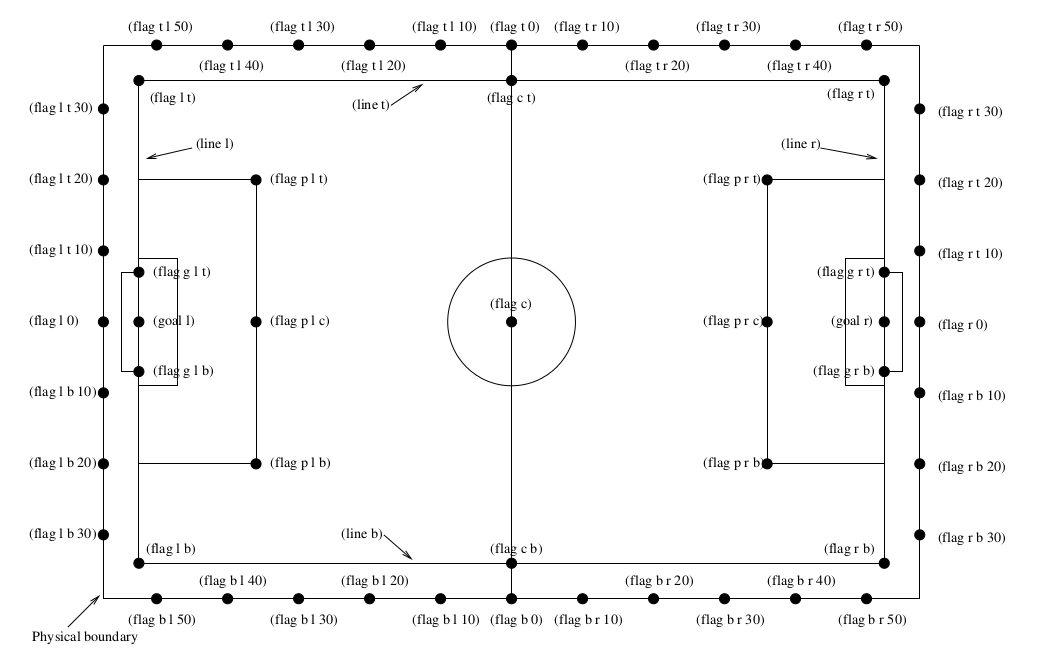
\includegraphics[width=150mm]{./graficos/flags.png}
\caption{Banderas en el campo de juego} \label{fig:flags}
\end{figure}

Además del sensor de visión, tenemos otro sensor de cuerpo que reporta el estado físico del jugador. Por ejemplo la estamina (necesaria para correr), la velocidad, el ángulo de la cabeza.


\section{Consideraciones finales}

En resumen, los problemas son que tenemos 11 agentes que deben jugar juntos con una capacidad limitada de comunicación. Que la representación del mundo, a pesar de ser de alto nivel, es muy compleja. Las acciones son continuas y además hay que controlar un gran número de parámetros que afectan cómo los agentes perciben el mundo. En los siguientes capítulos veremos conceptos que poco a poco nos llevarán a la resolución de este problema en la propuesta.
\chapter{Marco teórico}

En esta sección se describirán varios conceptos que serán útiles en el desarrollo de las siguientes secciones.

\section{Reinforcement Learning}

Es un área del aprendizaje automático, que se inspira en la psicología conductista. Básicamente consiste en qué acción debe seleccionar un agente dentro de un entorno para maximizar una recompensa en el largo plazo. El medio ambiente es normalmente modelado como un \ac{MDP}. El planteamiento de un problema en \ac{RL} siempre consta de 3 partes: las sensaciones (que determinan los estados), las acciones, y los objetivos (que determinan las recompensas) \cite{sutton1998reinforcement}.

Los elementos de un \ac{RL} son:
\begin{itemize}
\item \textbf{Estados}, conjunto de características que indican como está el ambiente en cada momento
\item \textbf{Acciones}, acciones disponibles en cada estado que pueden modificar el ambiente
\item \textbf{Política}, mapea estados a acciones
\item \textbf{Función de recompensa}, define el objetivo. Mapea un estado o par de (estado, accion) a una recompensa
\item \textbf{Función de valor}, es un valor numérico que define que tan bueno es un estado o par de (estado, accion) a largo plazo
\end{itemize}

Siempre existe el problema de balancear la exploración con la explotación. Siendo que la explotación nos permite utilizar los conocimientos que ya tenemos para obtener la máxima recompensa, pero la exploración nos permite obtener un mejor conocimiento y así mejorar nuestras decisiones. Si sólo se hiciera exploración, no tendría sentido puesto que nunca se explotaría el conocimiento generado. Y si siempre se hiciera explotación, quedaríamos atorados en la toma de decisiones sub-óptimas. Lo ideal es que haya una alta tasa de exploración al comienzo y que esta vaya disminuyendo hasta un valor pequeño estable con el tiempo.

Los métodos tradicionales de \ac{RL} han utilizado tablas como función de valor para mantener el retorno estimado de cada estado. Ejemplos de tales técnicas son los métodos de Monte Carlo, diferencias temporales y Q-learning. Sin embargo cuando el espacio de estados es demasiado grande, estas técnicas son imposibles de aplicar y se necesita el uso de nuevos métodos que serán descritos en este trabajo.


\subsection{Retorno esperado}

El retorno esperado $G_t$ es la cantidad de recompensa futura que se puede esperar partiendo de un estado, como se puede ver en su fórmula en la ecuación \eqref{eq:retorno_esperado}, donde $R_t$ es la recompensa en el tiempo $t$ y $T$ es el último paso del episodio.

\begin{equation} \label{eq:retorno_esperado}
G_t = R_{t+1} + R_{t+2} + R_{t+3} + ... + R_T
\end{equation}

Para tareas continuas, no existe un último episodio $T$, por lo tanto necesitamos un concepto adicional, el descuento $\gamma$, tal que $0 \leq \gamma < 1$. En la ecuación \eqref{eq:retorno_esperado_descuento} se aprecia como con el valor de descuento se consigue dar mayor peso a las recompensas más cercanas en el tiempo que aquellas que se encuentran distantes.

\begin{equation} \label{eq:retorno_esperado_descuento}
G_t = R_{t+1} + \gamma R_{t+2} + \gamma^2 R_{t+3} + ... 
\end{equation}


\subsection{Generalized Policy Iteration}

La iteración de política consiste en dos procesos simultáneos que interactúan. Uno hace que la función de valor sea consistente con la política actual (evaluación de política), y el otro hace a la política ávara respecto a la función de valor actual (mejora de política). En la iteración de política, estos procesos se alternan, completándose uno antes de que el otro comience, pero esto no es realmente necesario.

Llamamos \ac{GPI} a la idea de dejar que ambos procesos, la evaluación de la política y la mejora de la política, interactúen, independientemente de la granularidad y otros detalles de los dos procesos \cite{van1978discounted}. El esquema general de \ac{GPI} esta ilustrado en la figura \ref{fig:gpi}.

\begin{figure}[htb]
\centering
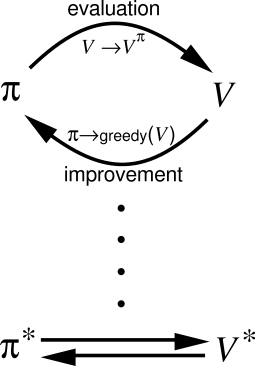
\includegraphics[width=40mm]{./graficos/gpi.png}
\caption{GPI} \label{fig:gpi}
\end{figure}


\subsection{On-policy vs Off-policy}

Los métodos on-policy tratan de evaluar y mejorar la política que está siendo usada para tomar decisiones. Imagine en cambio que queremos mejorar una determinada política $\pi$ estimando $v_\pi$ o $q_\pi$; pero sólo disponemos de episodios generados por otra política $\mu \neq \pi$. Llamamos a $\pi$ la política objetivo, porque aprender su función de valor es el objetivo del proceso de aprendizaje, mientras que a $\mu$ la llamamos política de comportamiento porque es la política que controla al agente y genera el comportamiento \cite{precup2001off}.


\subsection{Método actor-critic}

Consiste en tener una estructura de memoria separada para representar explícitamente la política independientemente de la función de valor. La estructura de la política es conocida como el actor, porque se usa para seleccionar acciones, y la función estimada de valor es conocida como el crítico, porque critica las acciones hechas por el actor \cite{barto2004j}.

Las críticas toman la forma del error, por ejemplo, en el caso de diferencias temporales, la crítica sería:

\begin{equation} \label{eq:critica_td}
\delta_t = R_{t+1} + \gamma V(S_{t+1}) - V(S_t)
\end{equation}

Donde $V$ es la función de valor actual implementada por el crítico. Este error puede ser usado para evaluar la acción recién tomada $A_t$. Si el error es positivo, la tendencia a seleccionar $A_t$ debería incrementar, pero si el error es negativo, dicha tendencia debería disminuir.


\subsection{Políticas parametrizadas}

Cuando el número de estados es demasiado grande, ya no es conveniente mantener promedios separados para cada uno en una tabla. En su lugar, el agente puede mantener la función de valor $v_\pi$ o $q_\pi$ como funciones parametrizadas y ajustar dichos parámetros para ajustarse mejor a los retornos observados. Esto también puede producir estimaciones precisas, aunque depende mucho del aproximador de función parametrizado que se escoja.


\subsection{Métodos de Gradiente de Política}

Son métodos de \ac{RL} que optimizan políticas parametrizadas respecto al retorno esperado usando la gradiente descendente \cite{sutton1999policy}.

Se asume que podemos modelar el sistema en forma de tiempo discreto y denotaremos el tiempo presente como $t$. Para tener en cuenta el factor estocástico del modelo, denotamos el cambio de estados usando una distribución de probabilidad $s_{t+1} \sim p(s_{t+1}|s_t, a_t)$ como modelo donde $a_t \in \mathbb{R}^N$ denota la acción actual, y $s_t, s_{t+1} \in \mathbb{R}^N$ denotan los estados actual y siguiente. También se asume que las acciones son generadas por una política $\pi(a_t|s_t)$ que se modela como una función de probabilidad para incorporar acciones exploratorias. Se asume que esta política está parametrizada por $k$ parámetros $\theta \in \mathbb{R}^k$. La secuencia de estados y acciones forman una trayectoria denotada por $\tau = [s_{0:H}, a_{0:H}]$ donde $H$ denota el horizonte que puede ser infinito. En cada instante de tiempo, el sistema recibe una recompensa denotada $r_t = r(s_t, a_t) \in \mathbb{R}$.

El objetivo general de la optimización de política en \ac{RL} es optimizar los parámetros de la política $\theta \in \mathbb{R}^k$ de forma que el retorno esperado se optimize.

\begin{equation}
J(\theta) = \left\lbrace \sum_{t=0}^H \gamma^t r_t \right\rbrace
\end{equation}

Para eso, los métodos de gradiente de política seguirán la gradiente ascendente del retorno esperado para actualizar los parámetros $\theta \in \mathbb{R}^k$.

\begin{equation}
\theta_{h+1} = \theta_h + \alpha_h \nabla_\theta J_{\theta = \theta_h}
\end{equation}

Donde $\alpha_h \in \mathbb{R}^+$ es la tasa de aprendizaje y $h = \{0,1,2,...\}$ es el número de la actualización actual. Nótese que el tiempo $t$ y el número de actualización $h$ son diferentes, por ejemplo, imagine un aprendizaje episódico donde la actualización se realiza sólo al final de cada episodio.


\section{Sistemas multiagente}

Un sistema multiagente es un sistema compuesto por múltiples agentes inteligentes que interactúan entre ellos. El bloque fundamental de construcción de los sistemas multiagente son los agentes, que aunque no tienen una definición formal y precisa, normalmente son vistos como entidades inteligentes, equivalentes en términos computacionales a un proceso del sistema operativo, que se pueden comunicar mediante un sistema de red.

Los agentes en un sistema multiagente tienen varias características importantes: La autonomía, visión local y descentralización, ya que no hay un agente de control designado.


\subsection{Aprendizaje en sistemas multiagente}

Sólo estudiaremos los modelos de aprendizaje con recompensa, ya que pueden ser modelados como un problema de \ac{RL}. Entre estos modelos de aprendizaje hay 4 tipos \cite{claus1998dynamics}:
\begin{itemize}
\item \textbf{Aprendizaje como un equipo}, donde los estados y las acciones incluyen a todos los agentes. De hecho se modela a todos los agentes como si fueran uno solo. Requiere de un programa centralizado que vea a todos los agentes como un todo y les indique qué hacer.
\item \textbf{Aprendizaje independiente}, donde todos los agentes conocen la ubicación de todos los agentes pero las acciones son individuales e independientes. Puede generar competición entre los agentes, llegando a un aprendizaje sub-óptimo.
\item \textbf{Aprendizaje de acciones conjuntas}, similar al aprendizaje independiente, pero involucra comunicación entre los agentes.
\item \textbf{Aprendizaje con valores de influencia}, los agentes pueden darse recompensas mutuamente para influenciar las acciones de los otros.
\end{itemize}


\section{Redes Neuronales y Deep Learning}

\subsection{Multilayer perceptron}

El \ac{MLP} es una red neuronal formada por mútliples capas que le permiten aproximar funciones no lineales \cite{yang2010multi}. La arquitectura del perceptron multicapa la podemos observar en la figura \ref{fig:mlp}.

\begin{figure}[htb]
\centering
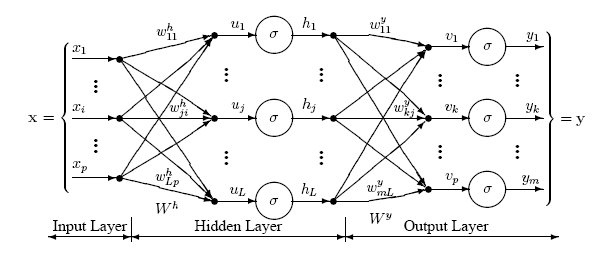
\includegraphics[width=150mm]{./graficos/mlp.jpg}
\caption{MLP} \label{fig:mlp}
\end{figure}

Básicamente tenemos entradas $x_i$ y salidas $y_i$. La red neuronal es una función paramétrica con parámetros $w$ que aproxima $y = f(x)$ modificando sus parámetros. Podemos ver a la red neuronal como una función $g(x, w) \sim f(x)$. El algoritmo que usa para aproximarse más a $f(x)$ es el de la gradiente descendente del error respecto a sus parámetros. El error puede ser cualquier función de error entre $f(x)$ y $g(x, w)$, siendo la más común la función de error cuadrático.

\begin{equation}
w = w - \alpha \nabla_w E
\end{equation}

\subsection{Restricted Boltzman Machine}

Las \ac{RBM} son redes neuronales generativas estocásticas que pueden aprender una distribución de probabilidad sobre su conjunto de entradas \cite{hinton2010practical}. La arquitectura de una \ac{RBM} se encuentra en la figura \ref{fig:rbm}. Consiste de nodos de unidades visibles $x$ y unidades escondidas $h$. Cada unidad visible está conectada a todas las unidades escondidas y viceversa. Cada conexión tiene un peso $w$ asociado, que es el parámetro que se busca optimizar mediante el entrenamiento. Cada unidad visible e invisible está desplazada por un bias $b$ o $c$. Las unidades visibles representan data observable mientras que las unidades escondidas describen las dependencias entre las variables observadas.

\begin{figure}[htb]
\centering
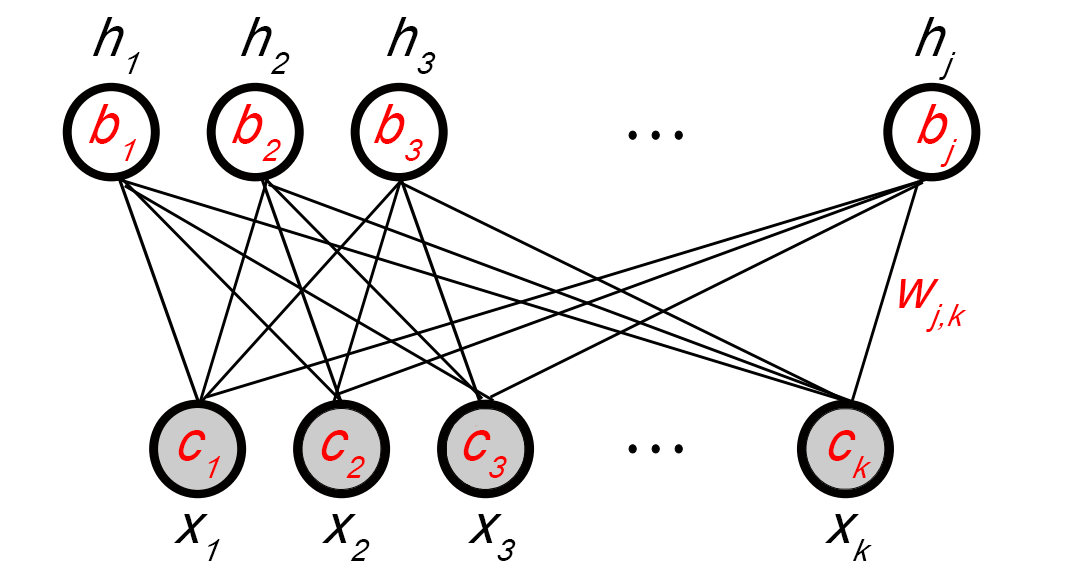
\includegraphics[width=100mm]{./graficos/rbm.png}
\caption{Arquitectura de la RBM} \label{fig:rbm}
\end{figure}

Para hallar las probabilidades se hace uso de una función de energía:

\begin{equation}
E(x, h) = -\sum_j \sum_k w_{j,k} h_j x_k - \sum_k c_k x_k - \sum_j b_j h_j
\end{equation}

El entrenamiento de esta red consiste básicamente en maximizar la probabilidad del valor de entrada. Para hacer esto se minimiza el promedio de la probabilidad logarítmica usando la gradiente descendente.


\subsection{Deep Belief Network}

En \cite{hinton2006reducing} se demostró que las \ac{RBM} podían ser apiladas y entrenadas de forma voraz para formar las llamadas Deep Belief Networks \cite{erhan2010does}. Las \ac{DBN} son modelos que aprenden a extraer una representación jerárquica profunda de los datos de entrenamiento. Modelan la distribución conjunta de un vector observado $x$ y las $l$ capas ocultas $h^k$ como sigue:

\begin{equation}
P(x, h^1, ..., h^k) = \left(\prod_{k=0}^{l-2} P(h^k|h^{k+1})\right) P(h^{l-1}, h^l)
\end{equation}

Donde $x = h^0$, $P(h^{k-1},h^k)$ es una distribución condicional para las unidades visibles condicionadas por las unidades ocultas de la \ac{RBM} en el nivel $k$, y $P(h^{l-1},h^l)$ es la distribución conjunta de las capas visible e invisible en el nivel más alto de la \ac{RBM}. Esto se ilustra en la figura \ref{fig:rbm_stack}

\begin{figure}[htb]
\centering
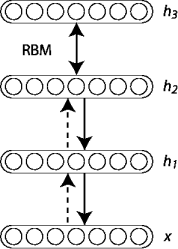
\includegraphics[width=40mm]{./graficos/rbm_stack.png}
\caption{Pila de RBM} \label{fig:rbm_stack}
\end{figure}

El principio de entrenamiento no supervisado goloso a nivel de capas puede ser aplicado a las \ac{DBN} con las \ac{RBM} como el bloque de construcción de cada capa \cite{hinton2006reducing, bengio2007greedy}. El proceso es como sigue:

\begin{enumerate}
\item Entrenar la primera capa como una \ac{RBM} que modela la entrada $x=h^0$ como su capa visible
\item Usar esta primera capa para obtener una representación de la entrada que será utilizada como data para la segunda capa. Existen dos soluciones comunes, escoger la representación como las activaciones promedio $p(h^1=1|h^0)$ o como muestras de $p(h^1|h^0)$
\item Entrenar la segunda capa como una \ac{RBM}, tomando la data transformada del paso anterior como ejemplos de entrenamiento para la capa visible de esa \ac{RBM}
\item Iterar (2 y 3) para el número deseado de capas, propagando haci arriba las muestras o activaciones promedio en cada paso
\item Ajuste fino de todos los parámetros de esta arquitectura profunda usando un criterio de aprendizaje supervisado. Por ejemplo, usando la gradiente descendente.
\end{enumerate}

\section{Consideraciones Finales}

En el siguiente capítulo veremos cómo estas ideas pueden ser usadas juntas para potenciarse mutuamente y crear un algoritmo de aprendizaje por refuerzo multiagente. Y a pesar de que surgen ciertas inconsistencias, estas son superadas con la introducción de nuevas estrategias que veremos a continuación.

\chapter{Estado del Arte}

\section{Agent2D}
\label{sec:agent2d}
Agent2D es un equipo de fútbol de muestra para la categoría de simulación 2D de la RoboCup. Forma parte del código base de HELIOS, un equipo que viene participando en competiciones de la RoboCup desde el año 2000. Ha ganado 2 veces el primer puesto y 2 veces el segundo puesto, y se ha mantenido entre los 3 primeros desde el 2007.

La primera vez que se publico el código base de HELIOS fue el 2006. Desde entonces está en constante mantenimiento. Este código es el más popular desde el 2012 y ha sido usado por un amplio número de equipos para participar por primera vez. En \cite{akiyama2013helios} podemos encontrar información más detallada sobre este programa.


\section{Deep Q Network}

Esta arquitectura aparece por primera vez en \cite{mnih2015human}. La idea básica es usar una Red Neuronal Profunda para aproximar la función de valor de las acciones. Con esta nueva arquitectura es posible aprender directamente de la información sensorial cruda. En este trabajo se usa una \ac{CNN} para leer directamente los píxeles de la pantalla de 49 juegos de atari. Sólo con esta información y el score se logra que el agente aprenda a jugar con desempeño sobrehumano en más de la mitad de los juegos.

Como usar aproximadores no lineales en \ac{RL} ha probado ser inestable, se aplican dos ideas clave:

\begin{itemize}
\item Usar un mecanismo biológicamente inspirado llamado replay de experiencias
\item Los valores objetivos son actualizados periodicamente, reduciendo así correlaciones 
\end{itemize}

A pesar de que con \ac{DQN} se pueden resolver problemas con estados de alta dimensionalidad; sólo puedo manejar acciones discretas y de baja dimensionalidad. Una solución obvia para adaptar \ac{DQN} a espacios de acciones continuas sería discretizar las acciones. Sin embargo esto tiene muchas limitaciones, especialmente la maldición de la dimensionalidad. Por ejemplo, en un sistema con 7 grados de libertad (como el brazo humano) con la discretización más gruesa $a_i \in {-k, 0, k}$, obtenemos un espacion de acciones con dimensionalidad $3^7=2187$.


\section{Deep Reinforcement Learning con espacio de acciones continuas}

En \cite{silver2014deterministic} se propone un algoritmo eficiente de \ac{RL} que puede ser aplicado con un espacio de acciones continuas. Este algoritmo usa la gradiente de una política determinista en un modelo actor-critic que permite usar otra política estocástica para lograr una exploración adecuada.

En \cite{lillicrap2015continuous} se hace lo mismo que en el trabajo anterior, pero mejora la estabilida del sistema utilizando los métodos de \ac{DQN}. Propone un algoritmo actor-critic libre de modelo, off-policy que utiliza aproximadores de funciones profundos para aprender políticas en espacios de acción continuos de varias dimensiones.
\chapter{Propuesta}

Se propone la creación de un equipo de fútbol para la categoría de simulación 2D de la RoboCup. Este equipo se implementará usando el algoritmo de aprendizaje por refuerzo \ac{DQN} y se espera que su desempeño sea por lo menos mejor que el equipo de muestra Agent2D que se explicó en la sección \ref{sec:agent2d}. La definición de los estados y acciones, así como la función de recompensa se encuentran en la siguiente sección.

\section{Definición de Estados, Acciones y Recompensas}

Los estados tendrán la siguiente información:

\begin{itemize}
\item $X_{jugador} \in [-54; 54]$ 
\item $Y_{jugador} \in [-32; 32]$
\item $dist_{balon} \in \mathbb{R}$
\item $dir_{balon} \in [-180; 180]$
\item Estamina $ \in [0; 4000]$
\item Esfuerzo $ \in [0; 1]$
\item Monto de velocidad $ \in \mathbb{R}^+$
\item Dirección de la velocidad $ \in [-180; 180]$
\end{itemize}

La información de los jugadores al rededor del agente se proporcionará haciendo un particionamiento de los 360º al rededor del agente en 10 porciones de 36º. A cada porción de 36º le corresponde una sección del estado:

\begin{itemize}
\item Equipo $ \in \{0, 1, 2\}$
\item Distancia $ \in \mathbb{R}^+$
\item Dirección del cuerpo $ \in [-180; 180]$
\item Dirección de la cabeza $ \in [-90; 90]$
\item Visto por última vez $ \in [0; 30]$
\end{itemize}

Se tienen 10 de estos bloques en un estado, uno por cada sección de 36º al rededor del jugador. Con esto, cada estado esta formado por 58 variables continuas, con lo cual queda justificado el uso de redes neuronales profundas.

Para las acciones también se tienen variables continuas, sin embargo se discretizarán para que puedan ser utilizadas con \ac{DQN}. Las posibles acciones son 34 en total:

\begin{itemize}
\item Girar $ \in \{-50, -20, -10, 10, 20, 50\}$
\item Acelerar $ \in \{10, 20, 50, 100\}$
\item Patear $ \in \{10, 20, 50, 100\} \times \{-50, -20, -10, 10, 20, 50\}$
\end{itemize}

También se necesita una función de recompensas, que en nuestro caso, funcionará en los siguientes casos:

\begin{itemize}
\item Gol a favor: +1
\item Gol en contra: -1
\end{itemize}

\section{Parámetros de la \ac{DQN}}

Para modelar la función de valor se utilizará una \ac{DBN} cuya entrada serán los estados definidos en la sección anterior. La salida de esta red neuronal profunda será una neurona de salida por cada una de las 34 acciones. En cada neurona de salida se tendrá el valor de la acción que corresponde a esa neurona. Se tendrá 2 capas ocultas con 50 neuronas en cada una. Además hay varios parámetros que aún falta definir, pero que se definirán en tiempo de implementación, como el tamaño de la memoria de replay, el factor de descuento, el tamaño de los batches, etc.
\chapter{Pruebas y Resultados}

A continuación se describirán las pruebas y resultados de trabajos similares, además de mostrar la planificación de pruebas para el presente trabajo.


\section{Pruebas y resultados en trabajos similares}

En \cite{mnih2015human} se usan como métricas el score promedio por episodio y el valor de acción promedio (Figura \ref{fig:dqn_results}). Luego se compara la eficiencia del agente de \ac{RL} con un jugador humano experto, siendo que el jugador humano tiene un 100\% de eficiencia, el agente de \ac{DQN} logra más de 100\% de eficiencia en 29 juegos de un total de 49 (Figura \ref{fig:dqn_vs_human}).

\begin{figure}[htb]
\centering
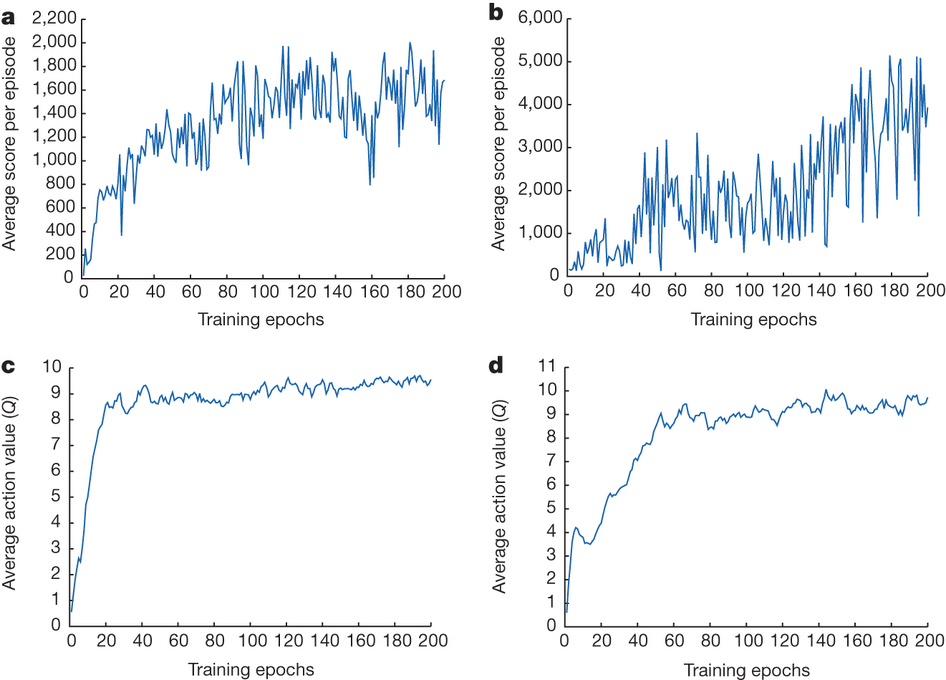
\includegraphics[width=150mm]{./graficos/dqn_results.jpg}
\caption{Resultados con DQN} \label{fig:dqn_results}
\end{figure}

\begin{figure}[htb]
\centering
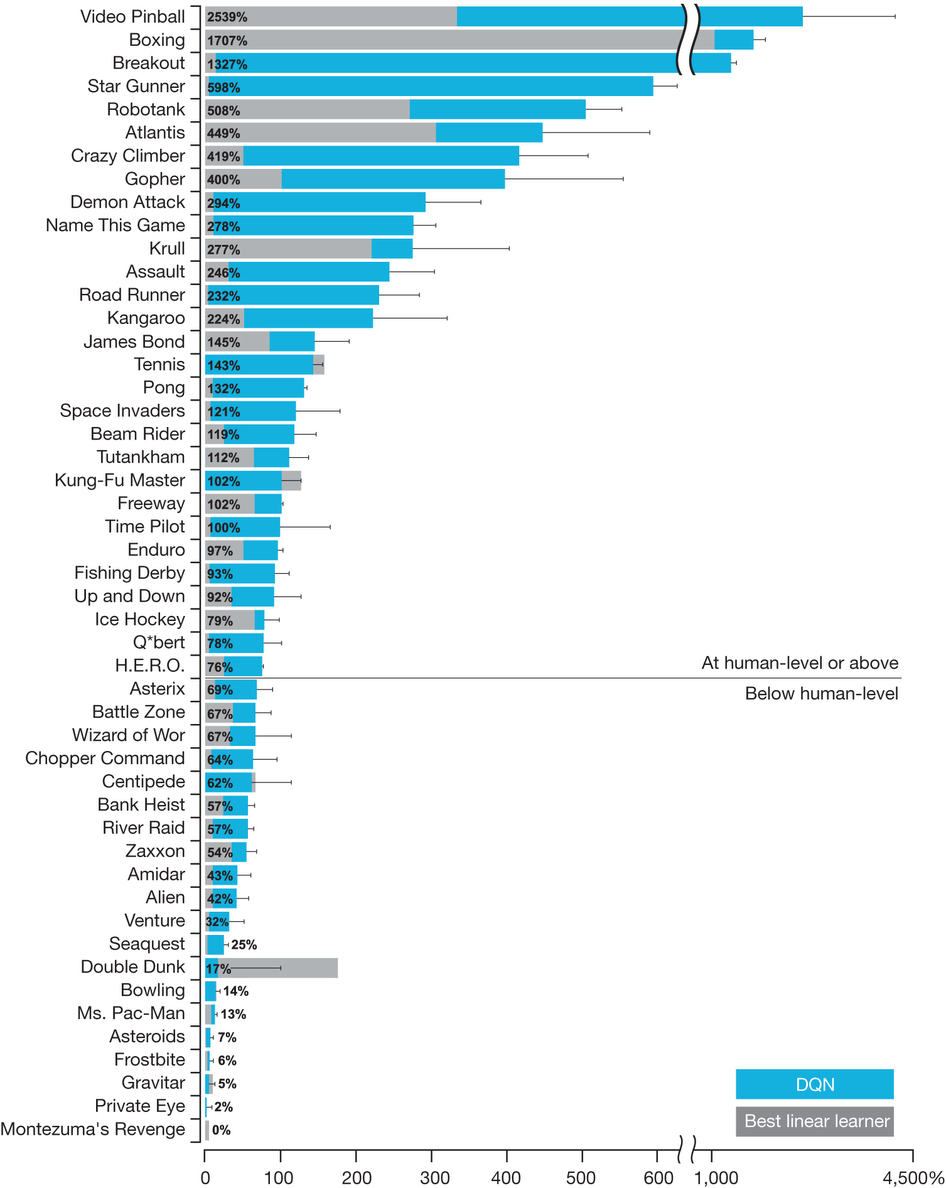
\includegraphics[width=150mm]{./graficos/dqn_vs_human.jpg}
\caption{DQN vs humano experto} \label{fig:dqn_vs_human}
\end{figure}

En \cite{silver2014deterministic} se usa una versión continua del problema de los bandidos para hacer una comparación directa entre las gradientes de política estocástica y deterministica. Luego se usan problemas donde el espacio de acciones es continuo y se comparan varios algoritmos recientes de \ac{RL} usando como métrica la recompensa total por episodio (Figura \ref{fig:dpg_results}).

\begin{figure}[htb]
\centering
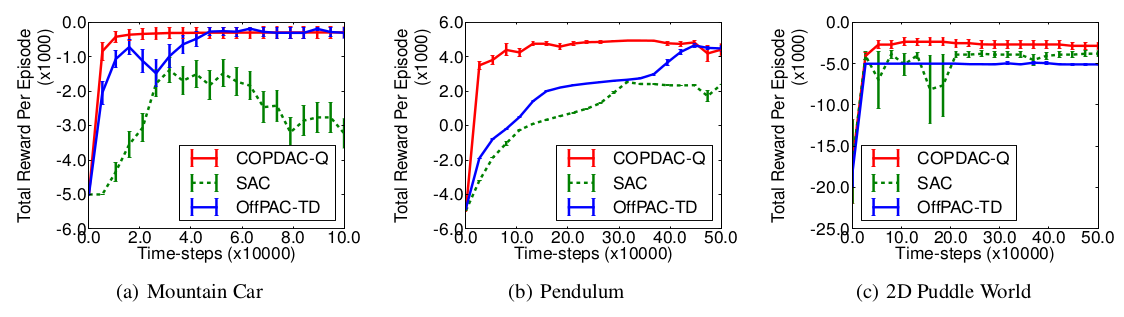
\includegraphics[width=150mm]{./graficos/dpg_results.png}
\caption{Resultados de \ac{DPG}} \label{fig:dpg_results}
\end{figure}

En \cite{lillicrap2015continuous} se utilizaron ambientes físicos simulados de varios niveles de dificultad para probar el algoritmo. Esto incluyo ambientes clásicos de \ac{RL} como cartpole, así como también tareas difíciles de alta dimensionalidad como brazos manipuladores o locomoción de esqueletos. Para la comparación se usa la recompensa normalizada (Figura \ref{fig:modified_dpg_results}).

\begin{figure}[htb]
\centering
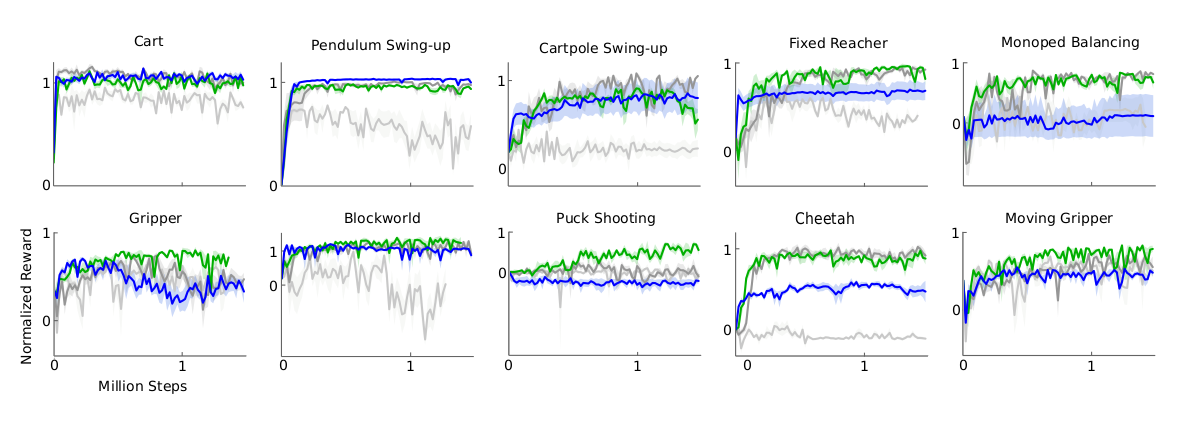
\includegraphics[width=150mm]{./graficos/modified_dpg_results.png}
\caption{Resultados de \ac{DPG} modificado} \label{fig:modified_dpg_results}
\end{figure}

\section{Planificación de pruebas}

Durante el entrenamiento del equipo se pretende registrar la recompensa por episodio, para evaluar la velocidad de convergencia.

Una vez que el equipo esté listo, se jugarán 50 partidos contra agent2D, registrando partidos ganados, perdidos y cantidad de goles. Si el número de partidos ganados es superior al 60\%, diremos que alcanzamos el objetivo.
\chapter{Conclusiones y Trabajos Futuros}\label{chap:conclusiones}

Se vio que los algoritmos de aprendizaje por refuerzo han recibido un impulso con la aparición de la Deep Q-Network, ya que nuevamente han llamado la atención de los investigadores y se están desarrollando varias líneas de investigación relacionadas con el tema. Una de esas líneas es la aplicación del aprendizaje por refuerzo en contextos con espacios de acciones continuas.

Con Deep Q-Network es posible calcular el valor de las acciones con una función paramétrica. Siendo las más comúnmente utilizadas las redes neuronales profundas, ya que permiten trabajar con grandes cantidades de estados continuos. Sin embargo, su aplicación no es trivial, ya que se generan inestailidades que se resuelven con la aplicación de dos ideas claves. La primera es usar una memoria de replay, y la segunda, actualizar los valores de las acciones periódicamente.

\section{Problemas encontrados}
Falta una mejor aplicación de las estrategias multiagente. Por ahora sólo se tiene un aprendizaje independiente.

\section{Recomendaciones}
Se recomienda utilizar un código base de alguno de los equipos ganadores de la categoría de simulación de la RoboCup de años pasados. Ya que la programación de un equipo básico, capaz de comunicarse y sincronizarse con el servidor, además de modelar el mundo, no es sencilla.

\section{Trabajos futuros}
Como trabajo futuro sería bueno implementar mejores estrategias de aprendizaje multiagente, como por ejemplo aprendizaje con valores de influencia.

%%%%%%%%%%%%%%%%%%%%%%%%%%%%%%%%%%%%%%%%%%%%%%%%%%%%%%%%%%%%%%%%%%%%%%

\bibliographystyle{apalike}
\bibliography{Bibliog}
\addcontentsline{toc}{chapter}{Bibliografía}

\end{document}
